\subsubsection{Base de datos}
\label{sec:base_datos}
Las sesiones, los pacientes y la configuración de la interfaz se almacenan en una base de datos relacional \textit{PostgreSQL} alojada en \textit{Supabase}, un servicio que agrega sobre la base un sistema de autenticación de usuarios y una interfaz de programación (API REST) generada automáticamente a partir del esquema. De esta forma la aplicación se comunica directamente con la base, sin un servidor intermedio propio, y el control de los permisos queda a cargo del propio motor de base de datos. La misma base es consultada por la página web pública del proyecto, que accede únicamente a las sesiones habilitadas para su difusión.

\paragraph{Modelo de datos.} La Figura~\ref{fig:der} presenta el diagrama entidad-relación de la base. Sus entidades son:
\begin{itemize}
    \item \texttt{patients}: cada paciente se identifica con un código anónimo correlativo (P-001, P-002, \dots). El nombre y el apellido se guardan solo para que el operador pueda reconocerlo al seleccionarlo, y no se incluyen en los datos exportados ni en la web pública.
    \item \texttt{sessions}: una fila por sesión de medición, asociada al paciente y al operador que la realizó. Guarda el número de sesión del paciente, la duración, las impedancias inicial y final (medianas del primer y del último minuto de medición), las notas y la calibración con la que se midió.
    \item \texttt{measurements}: las muestras de la sesión, con el instante según el reloj del equipo, la impedancia, la tasa de cambio y la tensión leída por el microcontrolador. Es la tabla de mayor volumen: una hora de medición genera alrededor de 14\,000 filas.
    \item \texttt{session\_events}: los eventos registrados durante la sesión (marcas, ingestas, micciones, microcortes, desconexiones y reconexiones), con su tipo, instante, impedancia y, cuando corresponde, el volumen en mililitros.
    \item \texttt{profiles}: el rol y el estado de aprobación de cada cuenta de operador. Se crea automáticamente cuando un usuario se registra en el sistema de autenticación (\texttt{auth.users}).
    \item \texttt{field\_definitions} y \texttt{calibrations}: catálogos que describen, respectivamente, las variables clínicas que se registran y las calibraciones del equipo.
\end{itemize}
Las muestras y los eventos dependen de su sesión, por lo que al eliminarse una sesión se eliminan con ella (borrado en cascada). En cambio, la eliminación de un paciente o de una cuenta no borra las sesiones asociadas, que se conservan sin esa referencia.

% Página apaisada: en vertical el diagrama queda con letra de ~4,5 pt.
% Dentro de sidewaysfigure \textwidth es el alto de la hoja; la altura se fija a mano
% para que entre en el ancho de texto (16 cm) junto con el epígrafe.
% Requiere \usepackage{rotating} en el preámbulo.
\begin{sidewaysfigure}
    \centering
    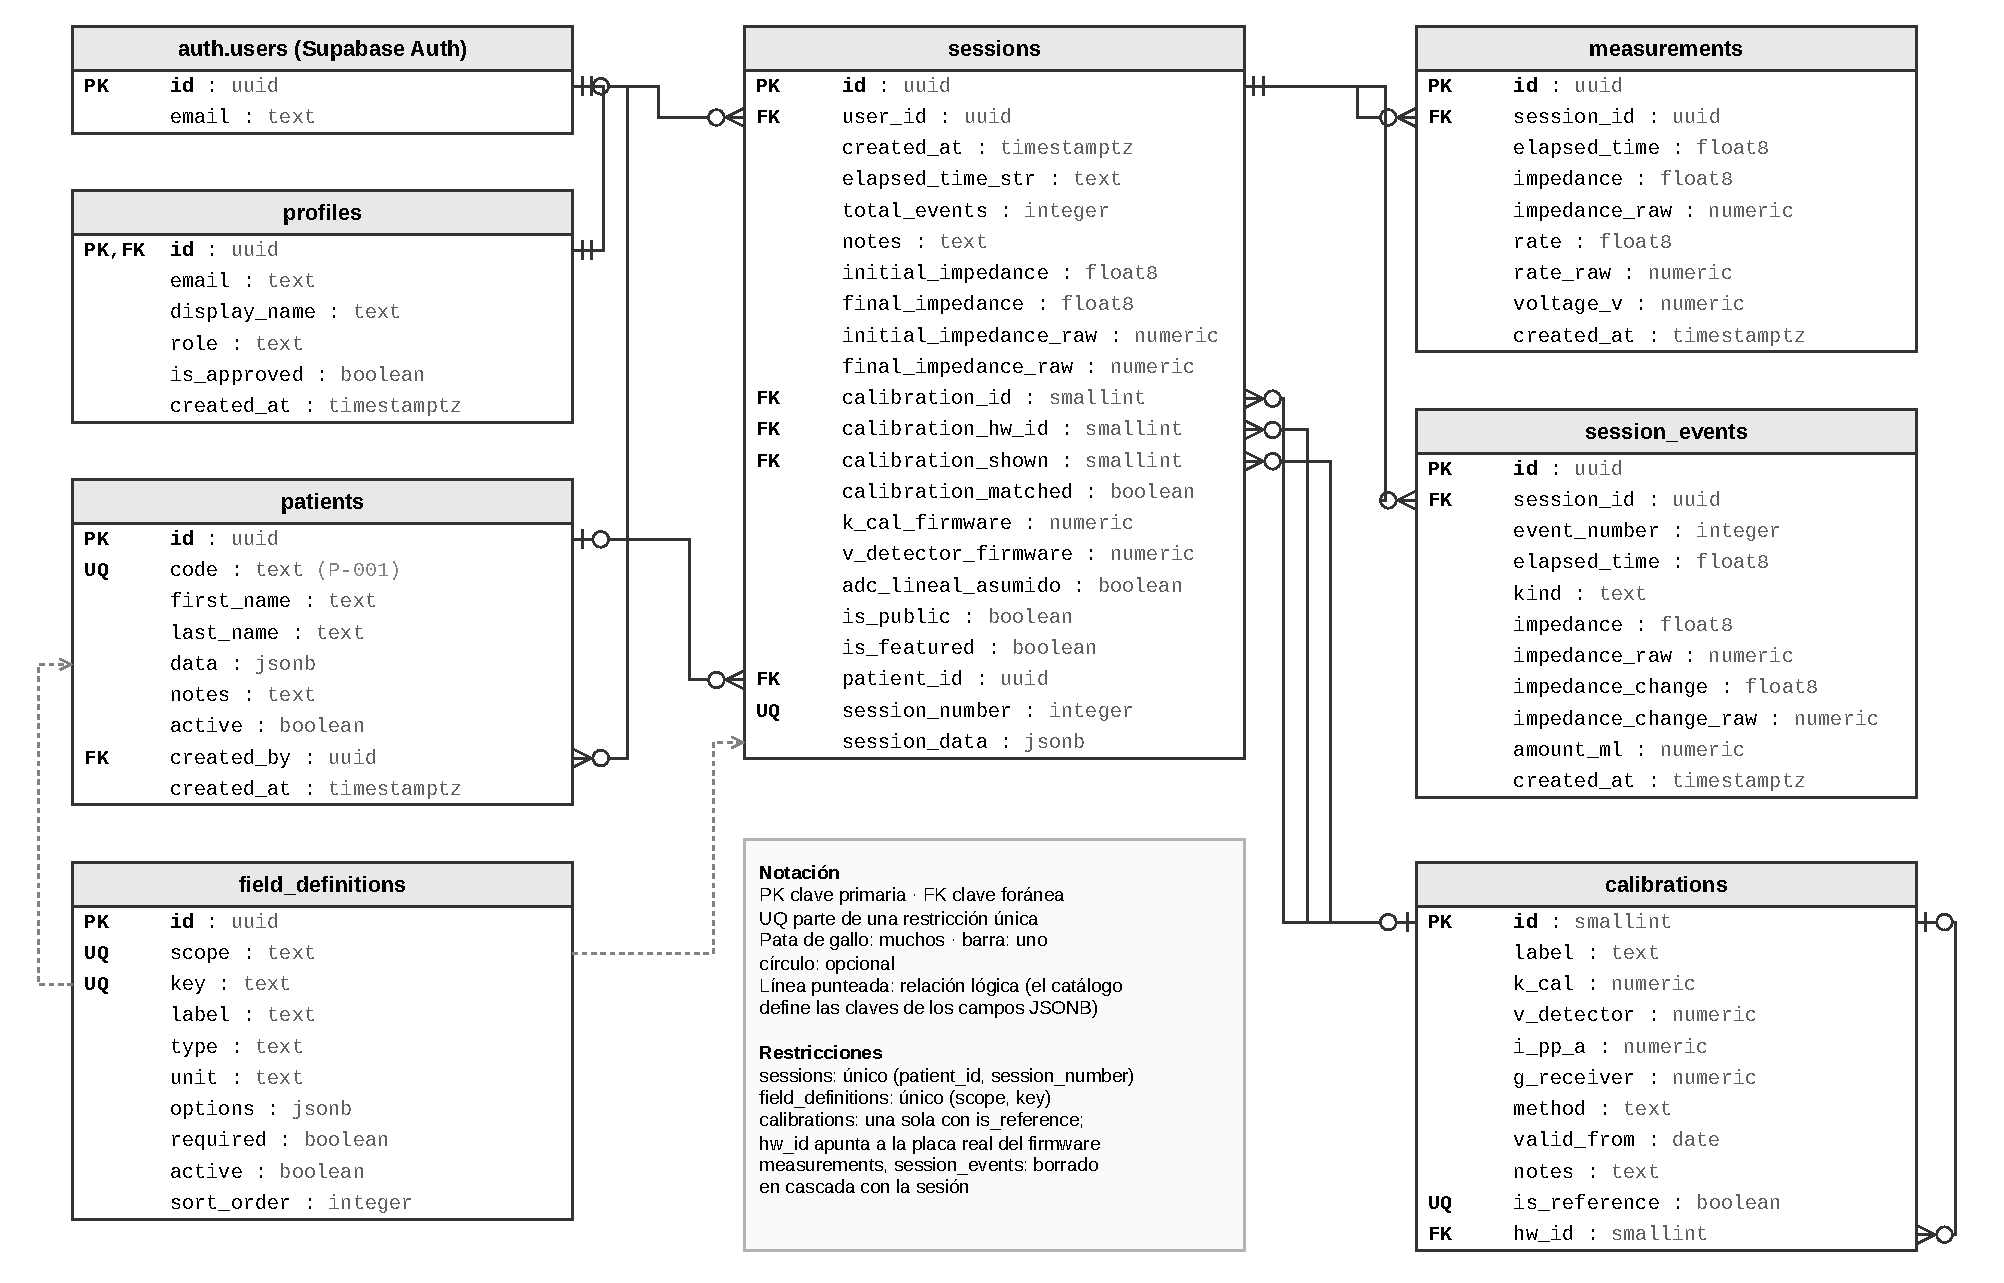
\includegraphics[width=\textwidth,height=14.5cm,keepaspectratio]{figuras/der_base_datos.pdf}
    \caption{Diagrama entidad-relación de la base de datos. Las relaciones en línea punteada son lógicas: el catálogo \texttt{field\_definitions} define las claves admitidas en los campos JSONB de pacientes y sesiones. Se omiten las columnas heredadas de versiones anteriores del esquema, que ya no se utilizan.}
    \label{fig:der}
\end{sidewaysfigure}

\paragraph{Variables configurables.} Las características de cada paciente y las condiciones de cada sesión no se almacenan en columnas fijas, sino en campos de tipo JSONB (\texttt{data} en pacientes y \texttt{session\_data} en sesiones), que admiten un conjunto variable de pares clave-valor. Las claves válidas, su tipo de dato (numérico, texto, fecha, booleano o lista de opciones), su unidad, su obligatoriedad y el orden en que se presentan se definen en el catálogo \texttt{field\_definitions}. La interfaz construye los formularios de carga a partir de este catálogo, por lo que incorporar una variable al protocolo se resuelve desde el panel de administración, sin modificar el esquema de la base ni distribuir una nueva versión de la aplicación.

\paragraph{Trazabilidad de la calibración.} Dado que la constante de calibración del equipo se corrigió a lo largo del proyecto, cada sesión registra con qué calibración fue medida. El catálogo \texttt{calibrations} guarda, para cada una, la constante $K_{CAL}$, la tensión del detector $V_{det}$, la corriente de excitación, la ganancia del receptor, el método con que se obtuvo y su fecha de vigencia, y señala una única calibración como referencia. Al iniciar la medición, el equipo informa la $K_{CAL}$ con la que opera; al guardar la sesión, un disparador (\textit{trigger}) de la base la busca en el catálogo y asocia la sesión a la calibración correspondiente. Si no se encuentra coincidencia, se asigna la calibración de referencia y la sesión queda marcada como no confirmada. Como una misma configuración del firmware puede corresponder a una placa cuya calibración medida es otra, se registran por separado la calibración del firmware (\texttt{calibration\_id}), la de la placa (\texttt{calibration\_hw\_id}) y la escala en la que están expresados los valores almacenados (\texttt{calibration\_shown}). También se identifican las sesiones registradas antes de corregir la lectura no lineal del conversor analógico-digital, cuya conversión es aproximada.

Los valores originales se conservan sin modificar en columnas con sufijo \texttt{\_raw}. Si una calibración se corrige, los datos se reescalan siempre a partir del valor original, por lo que la operación puede repetirse o revertirse sin pérdida de información. Siendo $Z = 2\,(V_{ADC} + V_{det})/K_{CAL}$, una impedancia $Z_a$ obtenida con la calibración $a$ se expresa en la calibración $b$ como
\begin{equation}
    Z_b = Z_a\,\frac{K_a}{K_b} + \frac{2\,(V_{det,b} - V_{det,a})}{K_b},
    \label{eq:reescalado}
\end{equation}
mientras que las diferencias de impedancia, como la variación respecto del basal, se escalan solo por el cociente $K_a/K_b$, ya que el término constante se cancela.

\paragraph{Integridad de los datos.} El número de cada sesión (1, 2, 3, \dots\ por paciente) lo asigna la base mediante un disparador y no la interfaz, de modo que resulta correlativo aunque las sesiones se registren desde distintas computadoras o se suban más tarde, por haberse medido sin conexión a internet. Para evitar que dos sesiones guardadas en simultáneo reciban el mismo número, el disparador toma un bloqueo exclusivo por paciente durante la asignación, y un índice único sobre el par paciente--número de sesión rechaza cualquier duplicado. Del mismo modo, los códigos de paciente son únicos y las claves foráneas impiden registrar muestras o eventos de sesiones inexistentes.

\paragraph{Seguridad.} La aplicación se conecta a la base con una clave pública que forma parte del ejecutable distribuido y que, por lo tanto, no puede considerarse secreta. Por este motivo el control de acceso no reside en la aplicación, sino en la propia base, mediante seguridad a nivel de fila (\textit{Row Level Security}, RLS): cada consulta se evalúa contra un conjunto de políticas que determinan qué filas puede leer o modificar el usuario autenticado. Las políticas definidas son:
\begin{itemize}
    \item Sin iniciar sesión no es posible acceder a ninguna tabla.
    \item Las cuentas nuevas quedan pendientes y, hasta ser aprobadas por un administrador, no acceden a los pacientes ni al catálogo de variables. Un disparador impide que un usuario se apruebe a sí mismo o modifique su propio rol.
    \item Cada operador accede únicamente a las sesiones que registró, junto con sus muestras y eventos, mientras que los administradores acceden a todas.
    \item Los catálogos de variables y de calibraciones pueden consultarse, pero solo los administradores pueden modificarlos.
    \item La web pública accede a través de vistas de solo lectura que exponen exclusivamente las sesiones habilitadas para su difusión, identificadas por el código del paciente.
\end{itemize}

\paragraph{Exportación del conjunto de datos.} Para el análisis de las mediciones, la base incluye una vista (\texttt{v\_dataset\_modelo}) que resume cada sesión en una fila: código del paciente, número de sesión, variables del paciente y de la sesión, impedancias inicial y final y su diferencia, calibración utilizada y si fue confirmada, cantidad de muestras, número y volumen total de ingestas y de micciones, y cantidad de microcortes, segundos perdidos y desconexiones. La vista se evalúa con los permisos de quien la consulta, por lo que respeta las mismas políticas de acceso que las tablas.

\paragraph{Respaldo y mantenimiento.} El esquema completo de la base y cada una de sus modificaciones se conservan como scripts SQL versionados junto con el código de la aplicación, lo que permite reconstruir la base desde cero. Antes de cualquier modificación se realiza una copia completa de las tablas en un esquema separado, inaccesible desde la API, y cada script se prueba previamente sobre una base de prueba construida con el mismo esquema. A la fecha de redacción, la base contiene 25 sesiones de 7 pacientes, con cerca de 300\,000 muestras.
